\documentclass[12pt, a4paper]{article}
\usepackage[utf8x]{inputenc}
\usepackage{ragged2e}
\usepackage{amsmath}
\usepackage{pdflscape}
\usepackage{graphicx}
\usepackage{hyperref}
\graphicspath{ {./images/} }
\usepackage{geometry}
\renewcommand{\contentsname}{İçindekiler Tablosu}
\usepackage[ddmmyyyy]{datetime}
\renewcommand{\dateseparator}{.}
\renewcommand{\figurename}{Şekil}
\renewcommand{\refname}{Referanslar}
\renewcommand{\tablename}{Tablo}
\geometry{
	top=2.5cm,
	left=2.5cm,
	right=2.5cm,
	bottom=2.5cm
}
% Title Page
\title{TRAFİKTE YORGUNLUK TESPİT SİSTEMİ DOKÜMANI}
\author{Sema YEŞİLKAYA}
\begin{document}
	\maketitle \newpage
	\tableofcontents{}  \newpage
\section{İlk Aşama: Gerekli Koşulların Belirlenmesi}
 \pagenumbering{arabic} 
 \subsection{Belirlenen Koşullar}
 \begin{itemize}
 	\item Sürücünün göz kapanma oranı
 	\item Sürücünün esnemesi
 	\item Sürücünün başının pozisyonu
 	\end{itemize}
 \subsection{Yöntemler}
 \begin{itemize}
 	
 	\item Yüz tanıma: Cascade \newline
 	Cascade yüz tanıma yöntemi, nesne tanıma alanında oldukça yaygın olarak kullanılan bir yöntemdir.
 	Temel olarak, bir yüzün farklı özelliklerini (gözler, burun, ağız vb.) tanımak için bir dizi önceden eğitilmiş sınıflandırıcıdan oluşur.
 	Bu sınıflandırıcılar, yüzün farklı bölgelerini tarar ve yüzün varlığını veya yokluğunu belirlemeye çalışır.
 	Cascade yöntemi, hızlı çalışma süresi ve yüksek doğruluk seviyeleri nedeniyle tercih edilir.
 	\item Tanınan yüzden gözleri ayırt etme : Cascade  \newline
 	Cascade yöntemi, yüz tanıma işlemi sırasında gözleri ayırt etmek için de kullanılır.
 	Gözleri ayırt etmek için yine önceden eğitilmiş sınıflandırıcılar kullanılır.
 	Bu sınıflandırıcılar, gözlerin varlığını veya yokluğunu tespit eder ve yüz tanıma sistemine daha fazla bilgi sağlar.
 	\item Göz durumlarının sınıflandırılması : SVM+ HOG  \newline
 	Destek vektör makinesi (Support Vector Machine,SVM), nesne tanıma ve sınıflandırma için kullanılır. Nesnelerin farklı bölümlerini (örneğin gözler, burun, ağız) tanımak için deformable part model kullanır.
 	HOG, nesnelerin kenarlarını ve şekillerini tanımak için kullanılır. Göz durumlarını sınıflandırmak için kullanılabilir.
 	\item Yorgunluk Tespiti : Perclos
 	Sürücülerin yorgunluk seviyelerini tespit etmek için kullanılır.
 	Sürücünün göz kapanma oranını (gözlerin ne kadar süreyle kapalı olduğunu) hesaplar.
 	Yüksek Perclos değerleri, sürücünün yorgun olduğunu ve dikkatinin dağıldığını gösterebilir. Yöntemler genel olarak \cite{ieeedata} baz alınarak belirlenmiştir.
 \end{itemize}
 	\begin{equation}\label{Perclos}
 		P = \frac{\text{kapalı göz içeren kare sayısı}}{\text{toplam kare sayısı}} \times 100
 	\end{equation}
 	Yukarıdaki (\ref{Perclos}) numaralı eşitlik Perclos değerinin nasıl hesaplanacağını gösterir.
  \begin{figure}[!h]
 	\centering
 	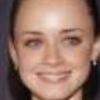
\includegraphics[width=14cm, height=7cm, keepaspectratio]{Alexis_Bledel_0001.jpg}
 	\caption{Veri setinden açık gözlü yüz örneği \cite{mrl}.}
 \end{figure}
  \begin{figure}[!h]
 	\centering
 	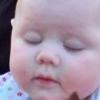
\includegraphics[width=17cm, height=7cm, keepaspectratio]{closed_eye_0047.jpg_face_2.jpg}
 	\caption{Veri setinden kapalı gözlü yüz örneği \cite{mrl}.} 
 \end{figure}\par
 	\subsection{Ana Kod}
 	
 	\begin{itemize}
 		\item import cv2: OpenCV kütüphanesini içe aktarır, bu kütüphane görüntü işleme işlevleri sağlar.
 		\item import dlib: Yüz tanıma ve yüz özelliklerini tespit etme işlevleri sağlayan bir kütüphane içe aktarır.
 		\item from scipy.spatial import distance: İki nokta arasındaki Öklid mesafesini hesaplamak için kullanılan bir fonksiyon içe aktarır.
 		\item calculate EAR fonksiyonu: Gözün iç ve dış köşeleri ile üst ve alt kapakları arasındaki mesafeleri hesaplar ve gözün açıklık oranını (EAR) döndürür.
 		\item Ana döngü (while True): Kamera görüntüsünü okur ve griye çevirir.
 		\item hog face detector ile yüzleri tespit eder.\item Her tespit edilen yüz için, dlib facelandmark ile yüz özelliklerini (68 nokta) bulur. ı\item Sol ve sağ göz için özellik noktalarını toplar ve gözlerin EAR değerlerini hesaplar. Eğer DİS değeri 0.26’dan düşükse, kişinin uykulu olduğunu varsayar ve ekrana “DROWSY” ve “Are you Sleepy?” yazılarını çizer.DİS değerini konsola yazdırır.\item “Are you Sleepy” adlı pencereyi gösterir. ESC tuşuna basıldığında döngüyü kırar ve kamerayı serbest bırakır, tüm pencereleri kapatır.
 	  
 	\end{itemize} 
 \section{İkinci Aşama: Haar Cascade Sınıflandırıcı Kullanma} 
 Bu hafta projelerde kullanabilmek için dlib kütüphanesini import etmem gerekti. Dlib yüz tanımlama gibi pek çok yerde kullanılan geniş kapsamlı ve açık kaynaklı bir kütüphane.\par Bilgisayarımda başka bir python sürümü kullanmam gerektiğini öğrendim ve bunu standart olarak kullanabilmek için path olarak ekledim. Fakat yine de olumlu bir sonuç elde edemedim. \begin{figure}[!h]
 	\centering
 	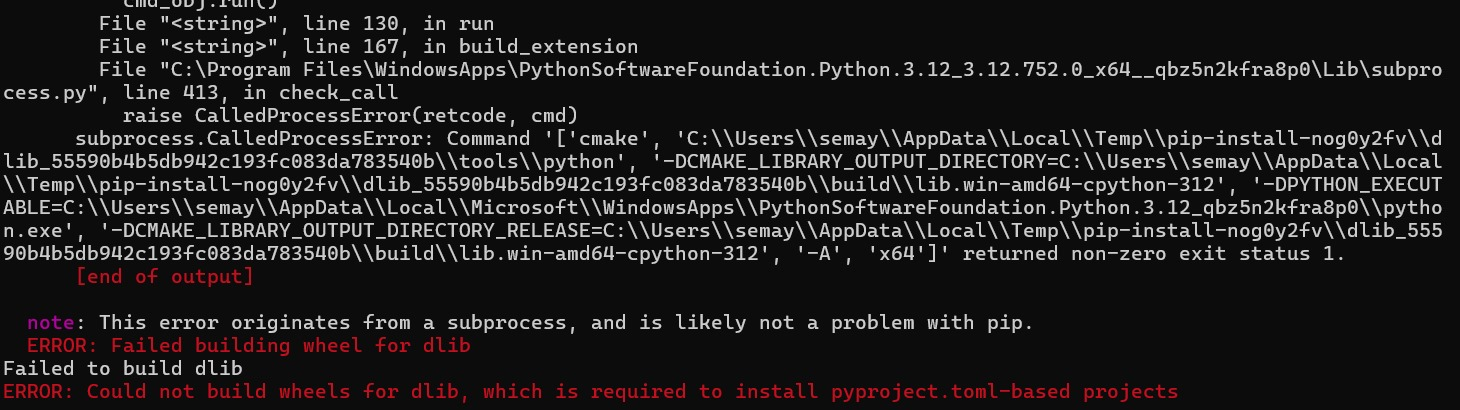
\includegraphics[width=17cm, height=7cm, keepaspectratio]{error.jpg}
 	\caption{Alınan hata.} 
 \end{figure}\par \begin{figure}[!h]
 	\centering
 	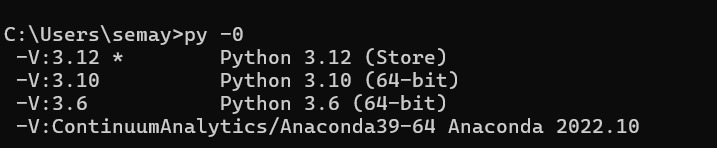
\includegraphics[width=17cm, height=7cm, keepaspectratio]{psurumu.jpg}
 	\caption{Python sürümleri.} 
 \end{figure}\par
 Bilgisayarımda yaşadığım sürüm uyuşmazlığını çözemediğim için dlib olmadan bu projenin nasıl yapıldığını araştırdım. Sadece Opencv import ederek yani import cv2 diyerek yapılan bir kod örneği inceledim ve haarcascade ile de çalışıldığını gördüm.\newline
 Haarcascade için hazır kodların yanında kendimiz de oluşturabiliriz. Pozitif ve negatif resimlere ihtiyacımız olur. Bu resimleri etikletleme işlemi gibi işlemden geçirdikten sonra bir tarafa nesnenin varlığını diğer tarafa olmadığını tanıtarak bu belgeler .bat formunda kaydedilir. Sistem tarafından çalıştırılıp tanınması için de .xml uzantısı olarak değiştirilir. Bu değişimi gerekli araçlarla yapabilirsiniz. Ben \cite{dasar_haartrain} burada anlatılan sistemi yararlı buldum ve ilerleyen süreçte bu veri setini kullanacağım.\clearpage
 \begin{figure}
 	\centering
 	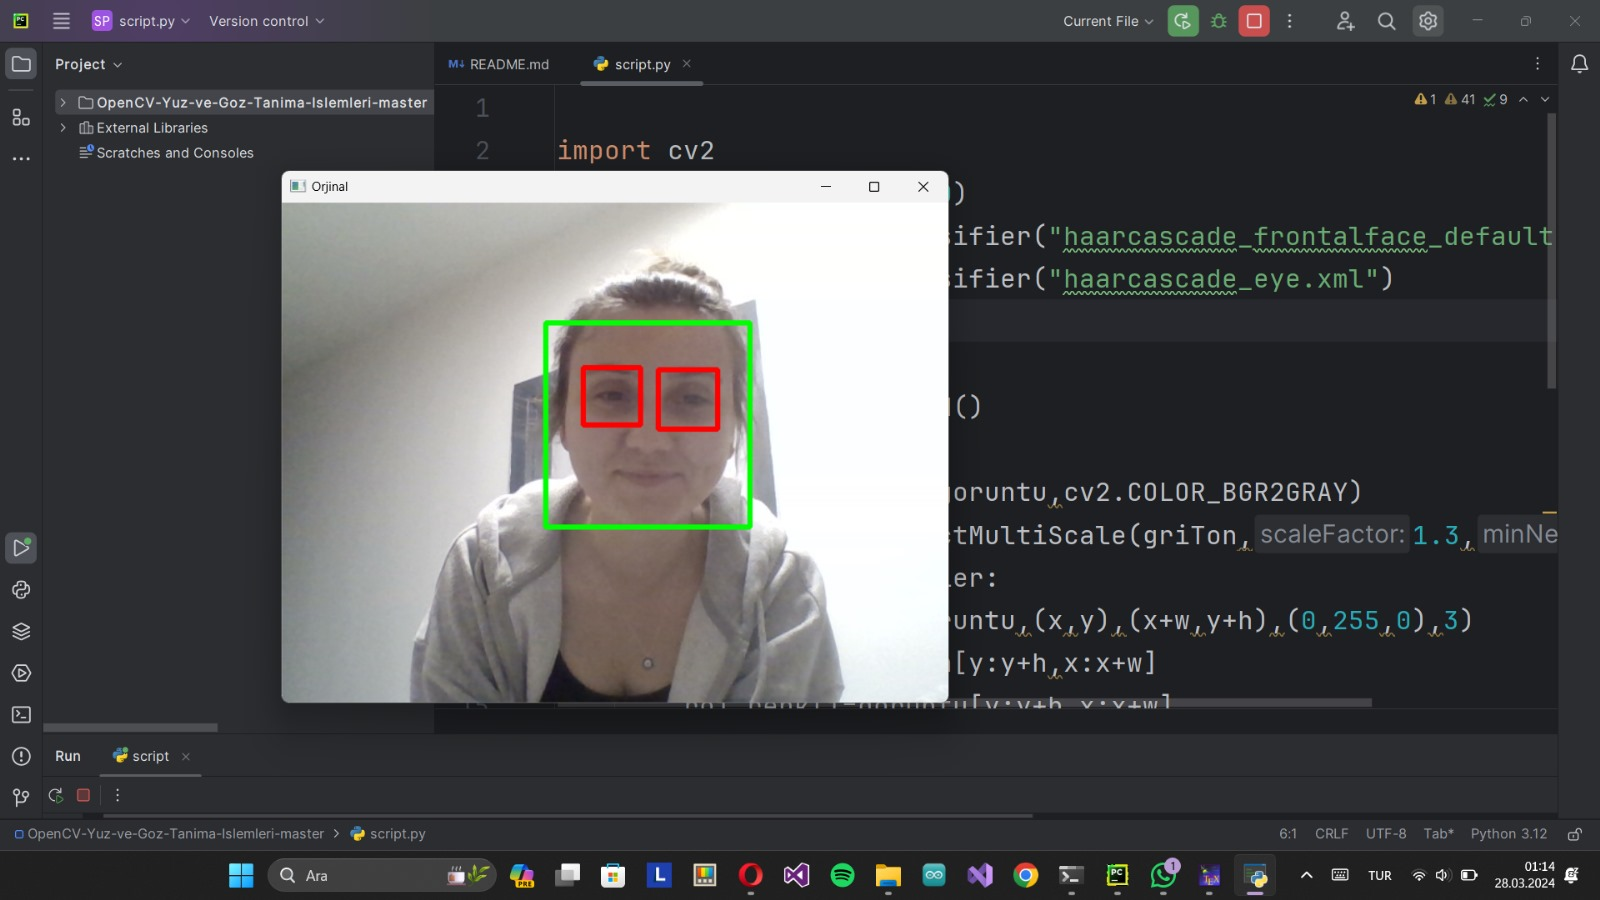
\includegraphics[width=17cm, height=7cm, keepaspectratio]{yuzgoztanima.jpg}
 	\caption{Yüz ve göz tespiti.} 
 \end{figure}
 \par
 Bu sisteme göz kapalılığını da eklemek istedim. Aslında bir sonraki hafta yapmam gerekn konu ama dlib yükleme süreci sebebiyle uzayacağını düşünüyorum. \\ Göz kapalılığını hesaplarken gözün etrafında bulunan 6 noktadan faydalanılır. Bu noktalar arası uzaklığını azalması ve belirli eşik değerin altında belirli bir süre kalması durumunda yorgunluk tespit edilmiş demektir. Bu duruma göre numpy ekledim ve hesaplama yaparak göz açıklık kapalılık kodunu yazmaya çalıştım. Kodun çalışması için dlib gerekiyormuş. Bu sebeple çalışmadı.
 \section{ Üçüncü Aşama: Göz Kapalılığı Tespiti} 
 Dlib kütüphanesini yüklemekle ilgili sorunum vardı ve bu sorunumu çözdüm. Sorunumu çözerken işlemlere baştan başladım. VsCode derleme araçlarını indirdim. Cmake kurdum. Daha sonra pip install dlib komutuyla bu kütüphaneyi indirdim \cite{onursahin}.İndirip örnek projelerde kullanmaya devam edebilirdim fakat ben dlib olmadan kullandığım projede denedim. Open- close durumlarında hata aldım.Dlib ile denemek istedim. Dlib kütüphanesinde landmark denen bir özellik vardır.Dlib kütüphanesindeki “landmark” terimi, yüzdeki belirli noktaları veya bölgeleri tanımlamak için kullanılır.Dlib’in en yaygın kullanılan yüz landmark dedektörü, 68 noktalı bir yapıya sahiptir ve yüzün ana hatlarını hızlı ve güvenilir bir şekilde tespit edebilir. \par Göz mesafesini hesaplamak için kullandığım standart olarak kullanılan eşik değerşu anlık bu ama değiştireceğim. Kullanıcıdan ilk önce gözünün açık ve kapalı hallerini isteyerek ona göre hesaplamaya geçilmesini düşünüyorum. \newpage
 \begin{figure}
 	\centering
 	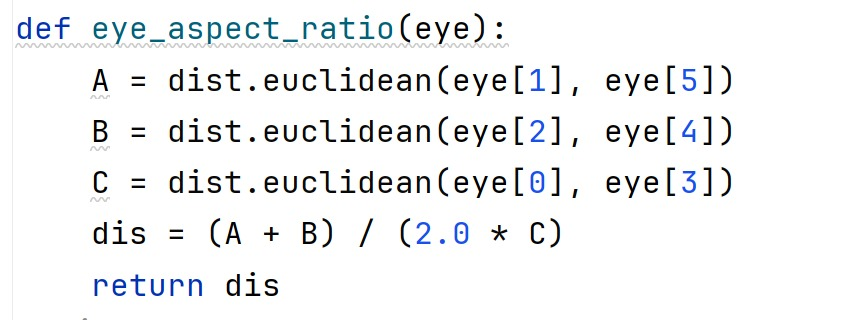
\includegraphics[width=10cm, height=7cm, keepaspectratio]{kod.jpg}
 	\caption{Göz mesafesi hesaplama.} 
 \end{figure} \par \begin{figure}[!h]
 	\centering
 	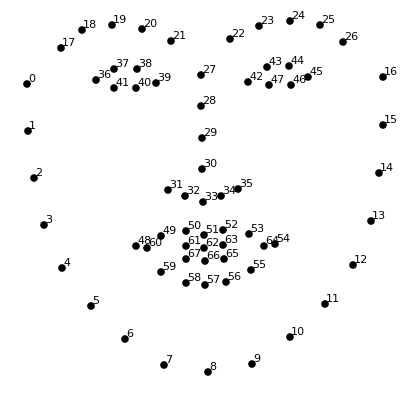
\includegraphics[width=17cm, height=7cm, keepaspectratio]{landmarks.jpg}
 	\caption{Göz tespiti için Dlib kütüphanesinin kullandığı landmark değerleri\cite{amos2018}.} 
 	\par
 \end{figure} 
 \section{ Dördüncü Aşama: Geleneksel Yöntem ile Yeni Yöntemin Karşılaştırılması} 
 Projede kullandığım yöntem geleneksel yöntemdi. Amacım, bu yöntem ile yeni teknolojilerden birini karşılaştırıp hangisinin daha sağlıklı sonuç verdiğini görmek.
 Yeni yöntem olarak CNN kullanılan bir örnek proje \cite{superthinking} buldum.
 CNN, yani Evrişimli Sinir Ağları (Convolutional Neural Networks), görüntü işlemede kullanılan bir derin öğrenme algoritmasıdır. Görselleri girdi olarak alır ve farklı operasyonlarla bu görsellerdeki özellikleri (features) yakalar ve sınıflandırır \cite{cnnnedir}. CNN, özellikle görüntü tanıma, nesne tespiti ve benzeri görsel tabanlı görevlerde etkili bir şekilde kullanılır.
 CNN’nin temel bileşenleri şunlardır:
 
Evrişim Katmanı (Convolutional Layer): Görüntü üzerinde gezinen ve özellikleri yakalayan filtreler içerir.\\
Aktivasyon Fonksiyonu (ReLU gibi): Modelin doğrusal olmayan özellikleri öğrenmesini sağlar.\\
Havuzlama Katmanı (Pooling Layer): Görüntü boyutunu küçültür ve özellikleri yoğunlaştırır.\\
Tam Bağlantılı Katman (Fully Connected Layer): Öğrenilen özellikleri kullanarak sınıflandırma yapar \cite{cnnnedirtek}.\par
 Bu katmanlar, bir görüntünün temel özelliklerinden daha karmaşık özelliklere kadar çeşitli soyutlama seviyelerinde özellikleri öğrenmek için bir arada çalışır. CNN modelleri, bu özellikleri öğrenmek ve güncellemek için eğitim sürecinde sürekli olarak kendilerini iyileştirir.\par
 \begin{figure}
 	\centering
 	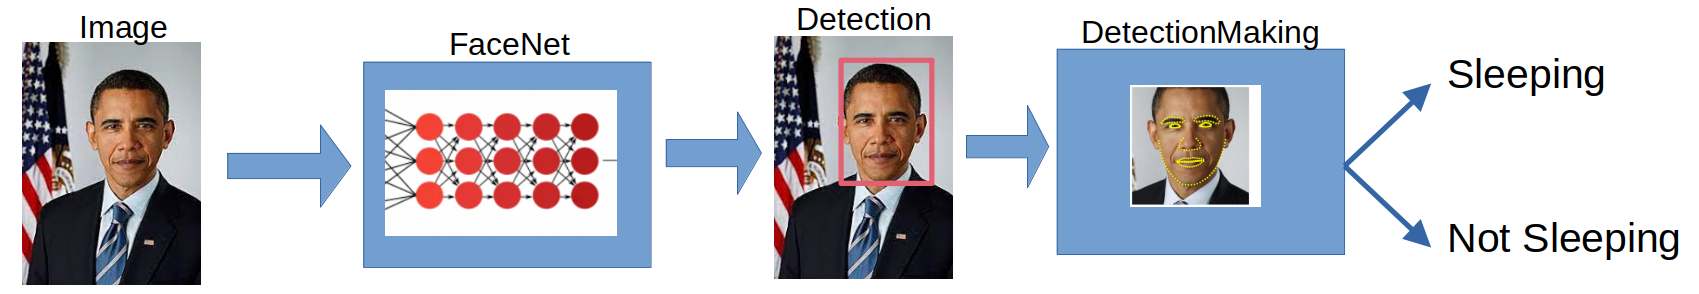
\includegraphics[width=10cm, height=7cm, keepaspectratio]{process.png}
 	\caption{CNN ile sürücü yorgunluğu tespiti \cite{eadali}.}
 \end{figure} 
 \begin{table}[h!]
 	\begin{center}
 		\caption{Haarcascade ve CNN Karşılaştırması.}
 		\label{tab:table1}
 		\begin{tabular}{l|c|c|}
 			\textbf{Özellik} & \textbf{Haarcascade} & \textbf{CNN}\\
 			\hline
 			Hızlı tespit süresi & Evet & Hayır\\
 			Düşük kaynak gereksinimi & Evet & Hayır\\
 			Yüksek doğruluk & Hayır & Evet\\
 			Özellik mühendisliği gerekmez & Hayır & Evet\\
 			Yüksek hesaplama gücü gereksinimi & Hayır & Evet\\
 			Uzun eğitim süresi & Hayır & Evet\\
 		\end{tabular}
 	\end{center}
 \end{table}
  Yukarıda gördüğünüz üzere CNN daha iyi bir sonuç çıkarıyor. Eğer doğruluğu önemsemeseydim Haarcascade kullanabilirdim.CNN ile yapılmış projede Tensorflow ve Theano yüklemesinde sorun yaşadığım için çalıştıramadım. Cascade için de başın pozisyonunu algılayıp üç boyutlu sisteme dönüştürerek vücut postürünü algılayan fonksiyon eklendi.\par 
  Yeni CNN kodunda Tenforflow sürüm hatası aldım. Thaeno kütüphanesini Numpy ile benzer olması dolayısıyla kaldırdım.Kod sahibi de Numpy kullanmıştı zaten.Ayrıca göz aralıklarını hesaplayarak gözün kapalı açık durumunu tespit ettiğimiz landmark olarak adlandırdığımız noktalar mantığında ve yine aynı yöntemle ağız açıklığını tespit eden fonksiyonu da eklyerek çoklu faktör kontrolü sağlandı. Bu değerlerden 3 veya daha fazlası gerçekleşiyorsa kişi yorgun olarak tanımlanım konumuna göre en yakın otele yönlendirme yapıyor.\newpage
   \begin{figure}
  	\centering
  	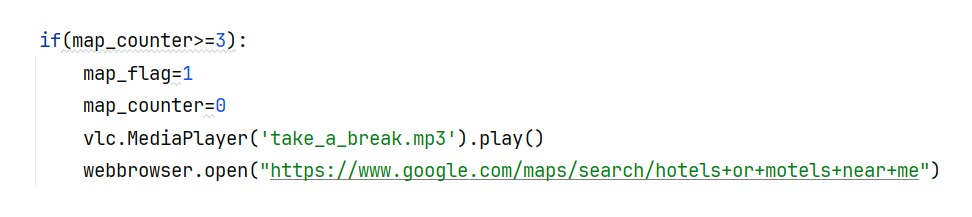
\includegraphics[width=10cm, height=7cm, keepaspectratio]{otel.jpg}
  	\caption{Yorgunluk eşiğine göre otele yönlendirme\cite{superthinking}.}
  \end{figure} 
   \begin{figure}
  	\centering
  	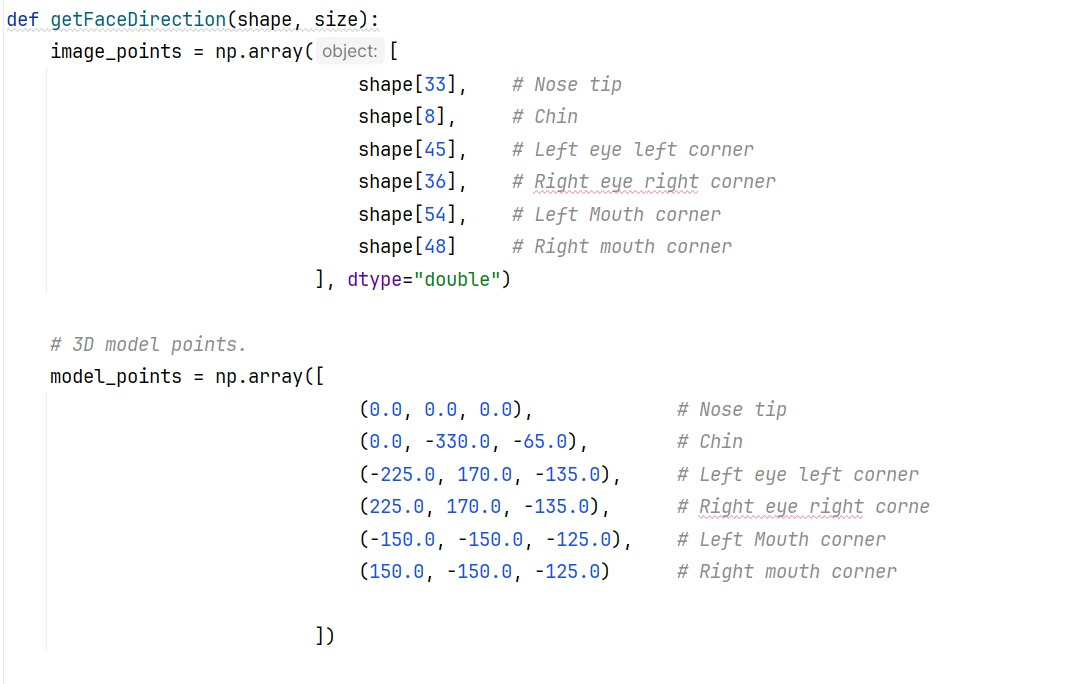
\includegraphics[width=10cm, height=7cm, keepaspectratio]{bastanimlama.jpg}
  	\caption{Baş pozisyonu tahmini için tanımlamalar\cite{superthinking}.}
  \end{figure}
  \section{ Sonuç} 
  Sonuç olarak projemde göz kapalılık durumu tespiti, ağza bakılarak uykululuk tespiti ve başın pozisyonuyla vücut duruşu tespiti sağladım. CNN'e bu kodlamaları geçirmeyi düşünüyorum. Çoğu yerde referans almıştım ve CNN e geçişte yine destek alsam da mantığı kendim kurarak ilerleyeceğim.
 	\bibliographystyle{ieeetr}
 	\bibliography{ref.bib} %\cite{aayushrai,bulentsezen,neelanjan00,researchgate,mrl,ieeedata,dasar_haartrain,amos2018,onursahin,eadali,superthinking,cnnnedir,cnnnedirtek}
 		\newpage
 	
  \end{document}
